% Architecture schematic of the current surrogate (xsum.models.surrogate.Surrogate, tier2=True).
% Compile: bash scripts/evaluate/render_schematic.sh. Update this file when the architecture changes.
\documentclass[tikz,border=6pt]{standalone}
\usetikzlibrary{positioning,fit,arrows.meta,calc,backgrounds}
\usepackage[T1]{fontenc}
\usepackage{amsmath,amssymb}
\usepackage{helvet}\renewcommand{\familydefault}{\sfdefault}
\definecolor{ink}{HTML}{222222}
\definecolor{paper}{HTML}{FFFFFF}
\definecolor{cin}{HTML}{0072B2}    % inputs
\definecolor{cenc}{HTML}{009E73}   % encoder
\definecolor{ccls}{HTML}{D55E00}   % classification heads
\definecolor{cgen}{HTML}{E69F00}   % generative heads
\definecolor{cout}{HTML}{555555}   % decoder / output
\definecolor{cbay}{HTML}{7B3294}   % Bayesian last layers (epistemic uncertainty)
\tikzset{
  box/.style={draw=ink, line width=1.2pt, rounded corners=3pt, fill=paper, align=left, inner sep=6pt, font=\small, text=ink},
  head/.style={box, text width=124mm},
  stage/.style={font=\footnotesize\bfseries, text=ink!80, anchor=south west},
  dim/.style={font=\scriptsize, text=ink!70},
  arr/.style={-{Latex[length=2.2mm]}, line width=0.7pt, draw=ink},
  arrd/.style={arr, dashed},
  arrc/.style={arr, dotted, line width=0.9pt},
}
\begin{document}
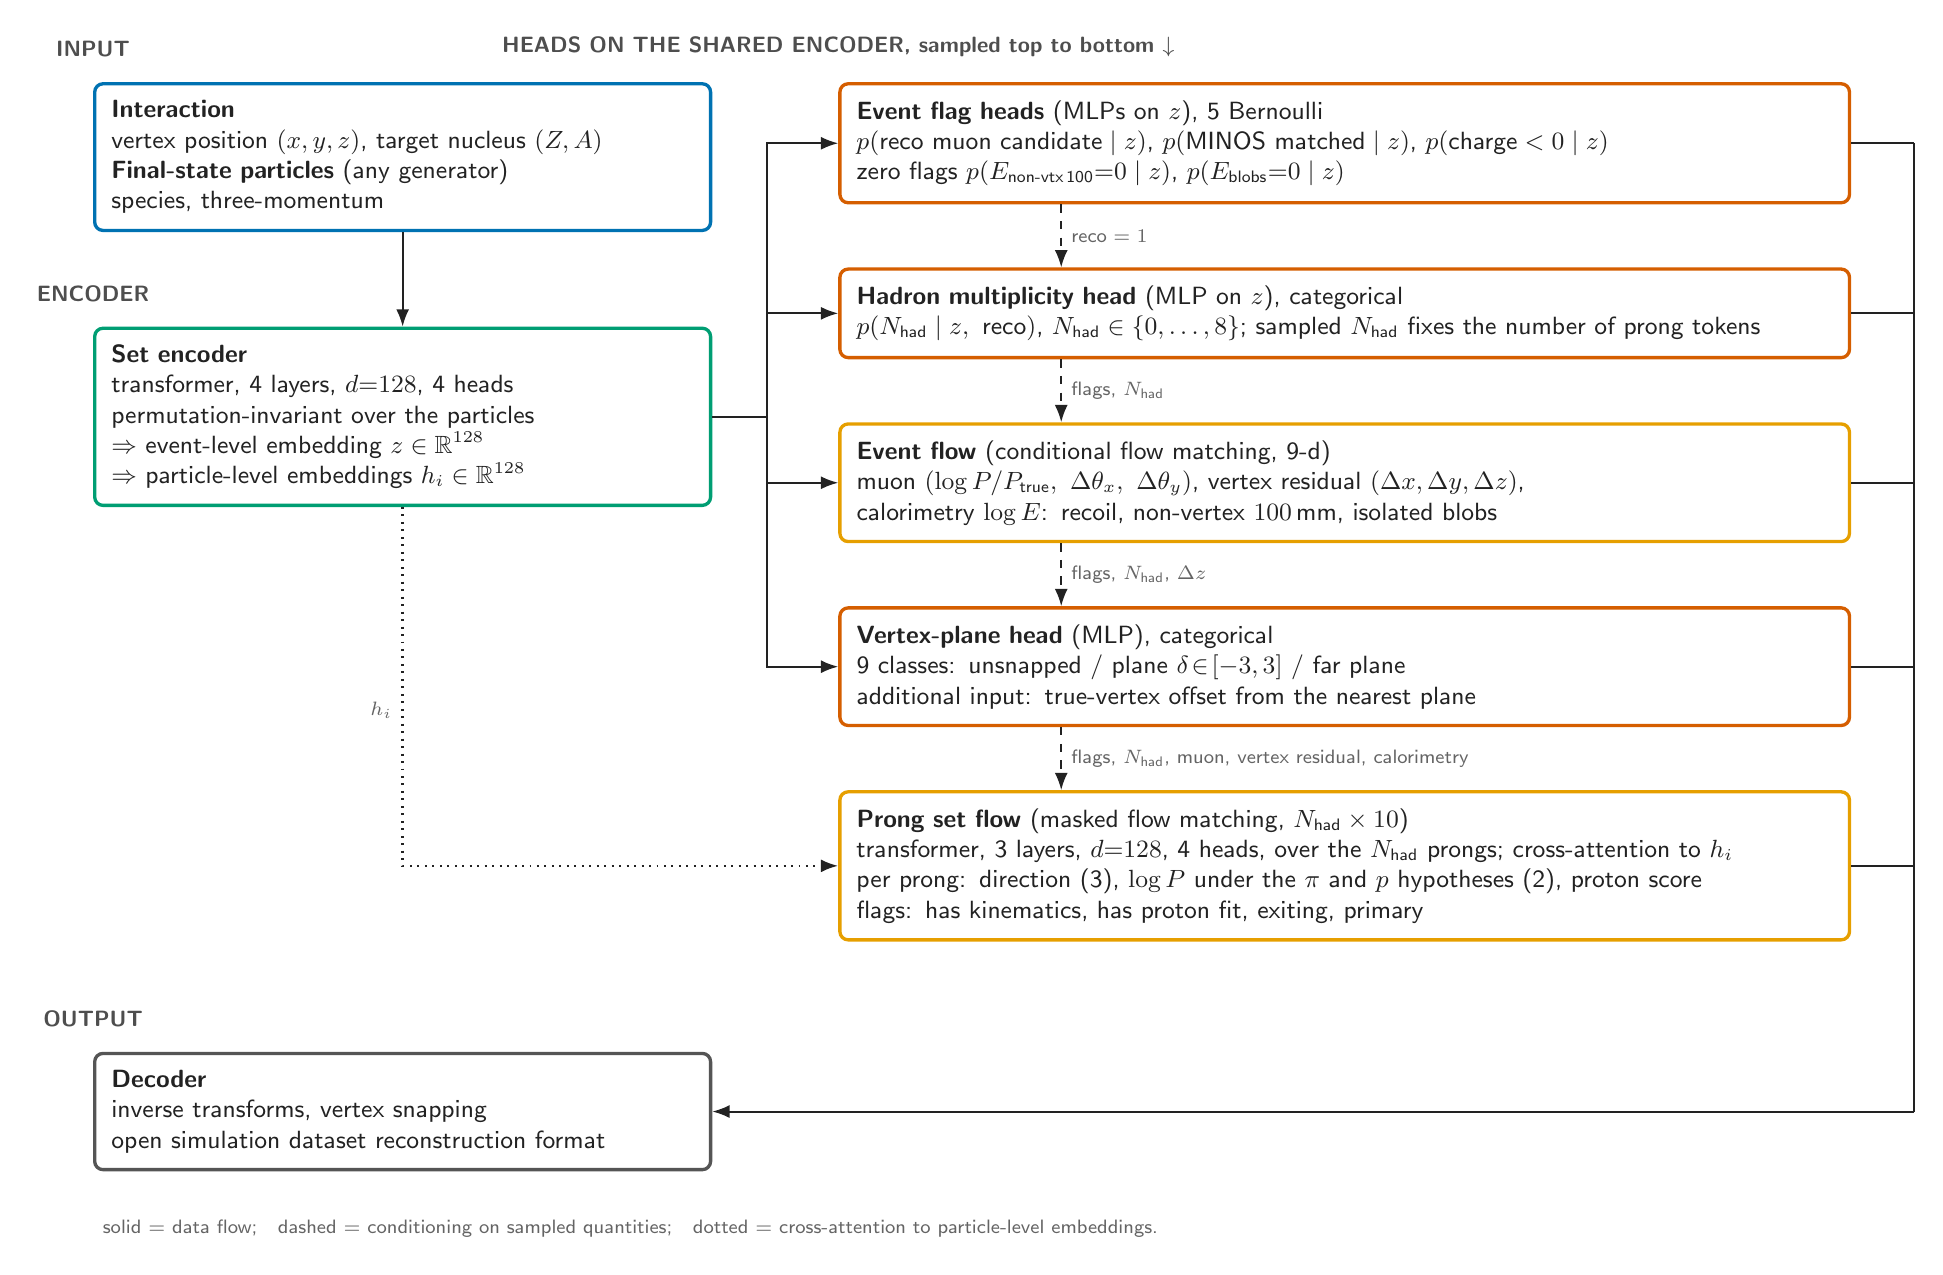
\begin{tikzpicture}[node distance=7mm and 9mm]

% ---------------- inputs and encoder (left column, top to bottom) ----------------
\node[box, draw=cin, text width=74mm] (gen) {\textbf{Interaction}\\
  vertex position $(x,y,z)$, target nucleus $(Z,A)$\\
  \textbf{Final-state particles} (any generator)\\
  species, three-momentum};
\node[box, draw=cenc, text width=74mm, below=12mm of gen.south west, anchor=north west] (enc) {\textbf{Set encoder}\\
  transformer, 4 layers, $d{=}128$, 4 heads\\
  permutation-invariant over the particles\\
  $\Rightarrow$ event-level embedding $z\in\mathbb{R}^{128}$\\
  $\Rightarrow$ particle-level embeddings $h_i\in\mathbb{R}^{128}$};

% ---------------- heads (right column, sampled top to bottom) ----------------
\node[head, draw=ccls, right=16mm of gen.north east, anchor=north west] (t0) {\textbf{Event flag heads} (MLPs on $z$), 5 Bernoulli\\
  $p(\text{reco muon candidate}\mid z)$, $p(\text{MINOS matched}\mid z)$, $p(\text{charge}<0\mid z)$\\
  zero flags $p(E_\text{non-vtx\,100}{=}0\mid z)$, $p(E_\text{blobs}{=}0\mid z)$};
\node[head, draw=ccls, below=8mm of t0.south west, anchor=north west] (card) {\textbf{Hadron multiplicity head} (MLP on $z$), categorical\\
  $p(N_\text{had}\mid z,\ \text{reco})$, $N_\text{had}\in\{0,\dots,8\}$; sampled $N_\text{had}$ fixes the number of prong tokens};
\node[head, draw=cgen, below=8mm of card.south west, anchor=north west] (t1) {\textbf{Event flow} (conditional flow matching, 9-d)\\
  muon $(\log P/P_\text{true},\ \Delta\theta_x,\ \Delta\theta_y)$, vertex residual $(\Delta x,\Delta y,\Delta z)$,\\
  calorimetry $\log E$: recoil, non-vertex $100$\,mm, isolated blobs};
\node[head, draw=ccls, below=8mm of t1.south west, anchor=north west] (vtx) {\textbf{Vertex-plane head} (MLP), categorical\\
  9 classes: unsnapped / plane $\delta\!\in\![-3,3]$ / far plane\\
  additional input: true-vertex offset from the nearest plane};
\node[head, draw=cgen, below=8mm of vtx.south west, anchor=north west] (t2) {\textbf{Prong set flow} (masked flow matching, $N_\text{had}\times 10$)\\
  transformer, 3 layers, $d{=}128$, 4 heads, over the $N_\text{had}$ prongs; cross-attention to $h_i$\\
  per prong: direction (3), $\log P$ under the $\pi$ and $p$ hypotheses (2), proton score\\
  flags: has kinematics, has proton fit, exiting, primary};

% ---------------- decoder (left column, bottom) ----------------
\node[box, draw=cout, text width=74mm, anchor=north west] (dec) at ($(enc.south west |- t2.south)+(0,-14mm)$) {\textbf{Decoder}\\
  inverse transforms, vertex snapping\\
  open simulation dataset reconstruction format};

% ---------------- arrows ----------------
\draw[arr] (gen.south) -- (enc.north);
\coordinate (fan) at ($(enc.east)+(7mm,0)$);
\foreach \h in {t0,card,t1,vtx} { \draw[arr] (enc.east) -- (fan) |- (\h.west); }
\draw[arrc] (enc.south) -- ++(0,-6mm) |- (t2.west) node[dim, pos=0.25, left] {$h_i$};
\draw[arrd] ([xshift=-36mm]t0.south) -- ([xshift=-36mm]card.north) node[dim, pos=0.5, right] {reco${}=1$};
\draw[arrd] ([xshift=-36mm]card.south) -- ([xshift=-36mm]t1.north) node[dim, pos=0.5, right] {flags, $N_\text{had}$};
\draw[arrd] ([xshift=-36mm]t1.south) -- ([xshift=-36mm]vtx.north) node[dim, pos=0.5, right] {flags, $N_\text{had}$, $\Delta z$};
\draw[arrd] ([xshift=-36mm]vtx.south) -- ([xshift=-36mm]t2.north) node[dim, pos=0.5, right] {flags, $N_\text{had}$, muon, vertex residual, calorimetry};
% outputs collected on a bus on the right, down and back to the decoder
\coordinate (bus) at ($(t0.east)+(8mm,0)$);
\foreach \h in {t0,card,t1,vtx,t2} { \draw[line width=0.7pt, draw=ink] (\h.east) -- (\h.east -| bus); }
\draw[line width=0.7pt, draw=ink] (t0.east -| bus) -- (bus |- dec.east);
\draw[arr] (bus |- dec.east) -- (dec.east);

% ---------------- stage labels ----------------
\node[stage, above=2mm of gen.north west] {INPUT};
\node[stage, above=2mm of enc.north west] {ENCODER};
\node[stage, above=2mm of t0.north west] {HEADS ON THE SHARED ENCODER, sampled top to bottom $\downarrow$};
\node[stage, above=2mm of dec.north west] {OUTPUT};

% ---------------- legend ----------------
\node[dim, below=5mm of dec.south west, anchor=north west, align=left] {
  solid $=$ data flow;\quad dashed $=$ conditioning on sampled quantities;\quad dotted $=$ cross-attention to particle-level embeddings.
};

\end{tikzpicture}
\end{document}
